\documentclass[10pt,twocolumn,letterpaper]{article}

%%%%%%%%% PAPER TYPE  - PLEASE UPDATE FOR FINAL VERSION
\usepackage[pagenumbers]{cvpr} % To force page numbers, e.g. for an arXiv version

% Include other packages here, before hyperref.
\usepackage{multirow}
\usepackage{multicol}
\usepackage{graphicx}
\usepackage{amsmath}
\usepackage{amssymb}
\usepackage{booktabs}
\usepackage[pagebackref,breaklinks,colorlinks]{hyperref}
\usepackage{marvosym}
\usepackage{ifsym}


% Support for easy cross-referencing
\usepackage[capitalize]{cleveref}
\crefname{figure}{图}{图}
\Crefname{figure}{图}{图}
\crefname{table}{表}{表}
\Crefname{table}{表}{表}
\crefname{section}{章节}{章节}
\Crefname{section}{章节}{章节}


%%%%%%%%% USER DEFINED MACROS
\newcommand{\yt}[1]{\textcolor{blue}{[yuntao: #1]}}
\newcommand\blfootnote[1]{%
  \begingroup
  \renewcommand\thefootnote{}\footnote{#1}%
  \addtocounter{footnote}{-1}%
  \endgroup
}


% Chinese support (auto-injected)
\usepackage{xeCJK}
\setCJKmainfont{Noto Serif CJK SC}[ItalicFont=AR PL UKai TW MBE]
\setCJKsansfont{Noto Sans CJK SC}
\setCJKmonofont{Noto Sans CJK SC}
\raggedbottom
\renewcommand{\figurename}{图}
\renewcommand{\tablename}{表}
\renewcommand{\abstractname}{摘要}
\renewcommand{\refname}{参考文献}
\begin{document}

%%%%%%%%% TITLE - PLEASE UPDATE
\title{BEVFormer v2：通过透视监督将现代图像骨干网络适配到鸟瞰视图识别（Adapting Modern Image Backbones to Bird's-Eye-View Recognition via Perspective Supervision）}

\author{Chenyu Yang\textsuperscript{\rm 1*} ~~ 
Yuntao Chen\textsuperscript{\rm 2*} ~~ 
Hao Tian\textsuperscript{\rm 3*} ~~ 
Chenxin Tao\textsuperscript{\rm 1} ~~ 
Xizhou Zhu\textsuperscript{\rm 3} ~~ 
Zhaoxiang Zhang\textsuperscript{\rm 2,4} \\
Gao Huang\textsuperscript{\rm 1} ~~ 
Hongyang Li\textsuperscript{\rm 5} ~~
Yu Qiao\textsuperscript{\rm 5} ~~
Lewei Lu\textsuperscript{\rm 3} ~~ 
Jie Zhou\textsuperscript{\rm 1} ~~
Jifeng Dai\textsuperscript{\rm 1,5\Letter}
\\ [0.15cm]
\textsuperscript{\rm 1}Tsinghua University ~~ 
\textsuperscript{\rm 2}Centre for Artificial Intelligence and Robotics, HKISI\_CAS \\ 
\textsuperscript{\rm 3}SenseTime Research ~~
\textsuperscript{\rm 4}Institute of Automation, Chinese Academy of Science (CASIA) \\
\textsuperscript{\rm 5}Shanghai Artificial Intelligence Laboratory
\\ [0.15cm]
{\tt\small \{yangcy19, tcx20\}@mails.tsinghua.edu.cn, chenyuntao08@gmail.com, tianhao2@senseauto.com}\\
{\tt\small \{zhuwalter, luotto\}@sensetime.com, zhaoxiang.zhang@ia.ac.cn}\\
{\tt\small \{gaohuang, jzhou, daijifeng\}@tsinghua.edu.cn, \{lihongyang, qiaoyu\}@pjlab.org.cn}
}

\maketitle

%%%%%%%%% ABSTRACT
\begin{abstract}
本文提出了一种带有透视监督（Perspective Supervision）的鸟瞰视图（BEV）检测器，收敛速度快且更适合现代图像骨干网络（Image Backbone）。现有当前最优（SOTA）的BEV检测器通常依赖于特定深度预训练的骨干网络（如 VoVNet），阻碍了蓬勃发展的图像骨干网络与BEV检测器之间的协同。为解决此限制，本文通过引入透视监督简化BEV检测器的优化。为此，本文提出一个两阶段（Two-stage）BEV检测器，将透视图头（Perspective Head）生成的提议（Proposals）送入鸟瞰视图头（BEV Head）进行最终预测。为评估模型有效性，本文开展了广泛的消融实验（Ablation Study），聚焦于监督形式及所提检测器的泛化性。该方法在多种传统与现代图像骨干网络上得到验证，并在大规模nuScenes数据集上取得新的SOTA结果。代码将很快开源。
\end{abstract}

\blfootnote{*: 同等贡献（Equal contribution）。}
\blfootnote{\Letter: 通讯作者（Corresponding author）。}

%%%%%%%%% BODY TEXT
\vspace{-5pt}
\section{引言}
鸟瞰视图（BEV）识别模型~\cite{OFT,pseudo-lidar,VPN,LSS,bevformer,CVT,PETR} 在自动驾驶领域引起了广泛关注，因为它们能够将来自多传感器的局部原始观测自然地整合到统一的三维输出空间中。
典型的BEV模型建立在图像骨干网络（Image Backbone）之上，后接一个视图变换（View Transformation）模块，将透视图特征（Perspective Feature）提升为BEV特征，再经由BEV特征编码器（Encoder）和任务特定头（Task-specific Head）进一步处理。
尽管大量工作致力于设计视图变换模块~\cite{CVT,LSS,bevformer} 并将不断增长的下游任务~\cite{LSS,fiery} 纳入新的识别框架中，BEV模型中图像骨干网络的研究却鲜受关注。
作为一个前沿且需求极高的领域，将现代图像骨干网络引入自动驾驶是自然而然的方向。
然而，研究社区仍坚持使用 VoVNet~\cite{Vovnet} 以享受其大规模深度预训练（Depth Pre-training）~\cite{DD3D} 带来的优势。
本文专注于释放现代图像特征提取器（Image Feature Extractor）在BEV识别中的全部潜力，为未来研究者在该领域探索更好的图像骨干网络设计打开大门。

然而，仅使用这些现代图像骨干网络而不进行适当的预训练无法产生满意的结果。
例如，在 ImageNet \cite{ImageNet} 上预训练的 ConvNeXt-XL \cite{ConvNext} 骨干网络在3D目标检测（3D Object Detection）上的表现仅与在 DDAD-15M 上预训练的 VoVNet-99 \cite{DD3D} 相当，尽管后者参数量是前者的3.5倍。
本文将现代图像骨干网络适配困难的原因归结为以下问题：
1) 自然图像与自动驾驶场景之间的领域差异。
在通用2D识别任务上预训练的骨干网络难以感知3D场景，尤其是深度估计（Depth Prediction）。
2) 当前BEV检测器复杂的结构。
以 BEVFormer~\cite{bevformer} 为例。3D边界框和物体类别标签的监督信号被视图编码器和物体解码器（Decoder）与图像骨干网络隔离开来，而每个编码器和解码器均由多层 Transformer 组成。
用于将通用2D图像骨干网络适配到自动驾驶任务的梯度流被堆叠的 Transformer 层扭曲。

为克服上述在将现代图像骨干网络适配到BEV识别中的困难，本文将透视监督（Perspective Supervision）引入 BEVFormer，即来自透视图任务的额外监督信号直接作用于骨干网络。
透视监督引导骨干网络学习2D识别任务中缺失的3D知识，并克服BEV检测器的复杂性，显著促进模型优化。
具体而言，本文在骨干网络上构建了一个透视3D检测头（Perspective 3D Detection Head）\cite{DD3D}，其以图像特征为输入并直接预测目标物体的3D边界框和类别标签。
该透视图头的损失（称为透视损失（Perspective Loss））作为辅助检测损失（Auxiliary Detection Loss），与来自BEV头的原始损失（BEV损失）相加。
两个检测头及其对应的损失项被联合训练。
此外，本文自然地将两个检测头结合成一个两阶段（Two-stage）BEV检测器——\textbf{BEVFormer v2}。
由于透视图头功能完整，能够在透视图上生成高质量的物体提议（Object Proposal），本文将其作为第一阶段提议。
将这些提议编码为物体查询（Object Query），与原始 BEVFormer 中的可学习查询合并，形成混合物体查询（Hybrid Object Query），再送入第二阶段检测头生成最终预测。

本文开展了广泛的实验来验证所提透视监督的有效性和必要性。
透视损失有助于图像骨干网络的适配，从而提升检测性能并加速模型收敛。
而若无此监督，即使采用更长的训练计划，模型也无法达到可比较的结果。
最终，本文成功将现代图像骨干网络适配到BEV模型中，在 nuScenes \cite{nuscenes} 测试集上达到63.4\% NDS。

本文贡献总结如下：
 \begin{itemize}
     \item 指出透视监督是将通用2D图像骨干网络适配到BEV模型的关键，通过透视图上的检测损失显式地添加此监督。
     \item 提出一种新颖的两阶段BEV检测器 BEVFormer v2，包含一个透视3D检测头和一个BEV检测头，前者的提议与后者的物体查询相结合。
     \item 通过与最新图像骨干网络结合，在 nuScenes 数据集上取得了相比先前SOTA结果的显著提升，验证了方法的有效性。
 \end{itemize}

\section{相关工作}
\subsection{BEV 3D目标检测器}
鸟瞰视图（BEV）目标检测（Object Detection）近年来受到越来越多的关注~\cite{OFT,VPN,pseudo-lidar,LSS,bevformer,CVT,PETR}，在自动驾驶系统中取得了巨大成功。

早期工作包括 OFT~\cite{OFT}、Pseudo LiDAR~\cite{pseudo-lidar} 和 VPN~\cite{VPN}，它们揭示了如何将透视图特征转换为BEV特征，但要么仅针对单摄像头，要么在不太知名的任务上评估。
OFT~\cite{OFT} 率先采用从2D图像特征到3D BEV特征的转换用于单目3D目标检测（Monocular 3D Object Detection）。
Pseudo LiDAR~\cite{pseudo-lidar} 顾名思义，通过单目深度估计（Monocular Depth Estimation）和相机内参创建伪点云，随后在BEV空间中进行处理。
VPN~\cite{VPN} 首次将多视角（Multi-view）相机输入融合为俯视图特征图用于语义分割（Semantic Segmentation）。

现代方法充分利用了2D-3D视图变换（View Transformation）提供的从不同透视图传感器整合特征的便利。
LSS~\cite{LSS} 通过引入潜在深度分布（Latent Depth Distribution）扩展了 OFT，用于BEV柱状特征的池化。此外，LSS 对六个环绕图像（而非 OFT 中的单张图像）进行了池化。
与 LSS 的2D到3D提升或 OFT 的3D到2D投影不同，CVT~\cite{CVT} 利用相机感知位置编码（Camera-aware Positional Encoding）和密集交叉注意力（Dense Cross Attention）连接透视图和BEV视图的特征。
PETR~\cite{PETR} 设计了一种无需显式BEV特征构建的方法，将透视图特征图与3D位置嵌入特征图逐元素融合，然后应用 DETR 风格的解码器（Decoder）进行目标检测。
BEVFormer~\cite{bevformer} 利用空间交叉注意力（Spatial Cross-attention）进行视图变换和时序自注意力（Temporal Self-attention）进行时序特征融合。BEVFormer 完全基于 Transformer 的结构使其BEV特征比其他方法更通用，能够轻松支持非均匀和非规则的采样网格。
此外，如 SimpleBEV~\cite{simplebev} 所示，多尺度可变形注意力（Multi-scale Deformable Attention）~\cite{deformable-detr} 在所有提升策略中表现最佳。
因此，本文选择基于 BEVFormer 构建检测器以利用上述优势。

除已发表的工作外，由于该领域的受欢迎程度，还有许多同期工作。
BEVDet~\cite{BEVDet} 引入了丰富的图像级和BEV级数据增强用于训练。
BEVStereo~\cite{bevstereo} 和 STS~\cite{STS} 均采用时序立体（Temporal Stereo）范式以获得更好的深度估计。
PolarFormer~\cite{polarformer} 提出了非笛卡尔（Non-cartesian）3D网格设置。
SimpleBEV~\cite{simplebev} 比较了不同的2D-3D提升方法。

与现有主要探索检测器设计的工作不同，本文专注于将现代图像骨干网络适配到BEV识别模型中。

\begin{figure*}[t]
    \centering
    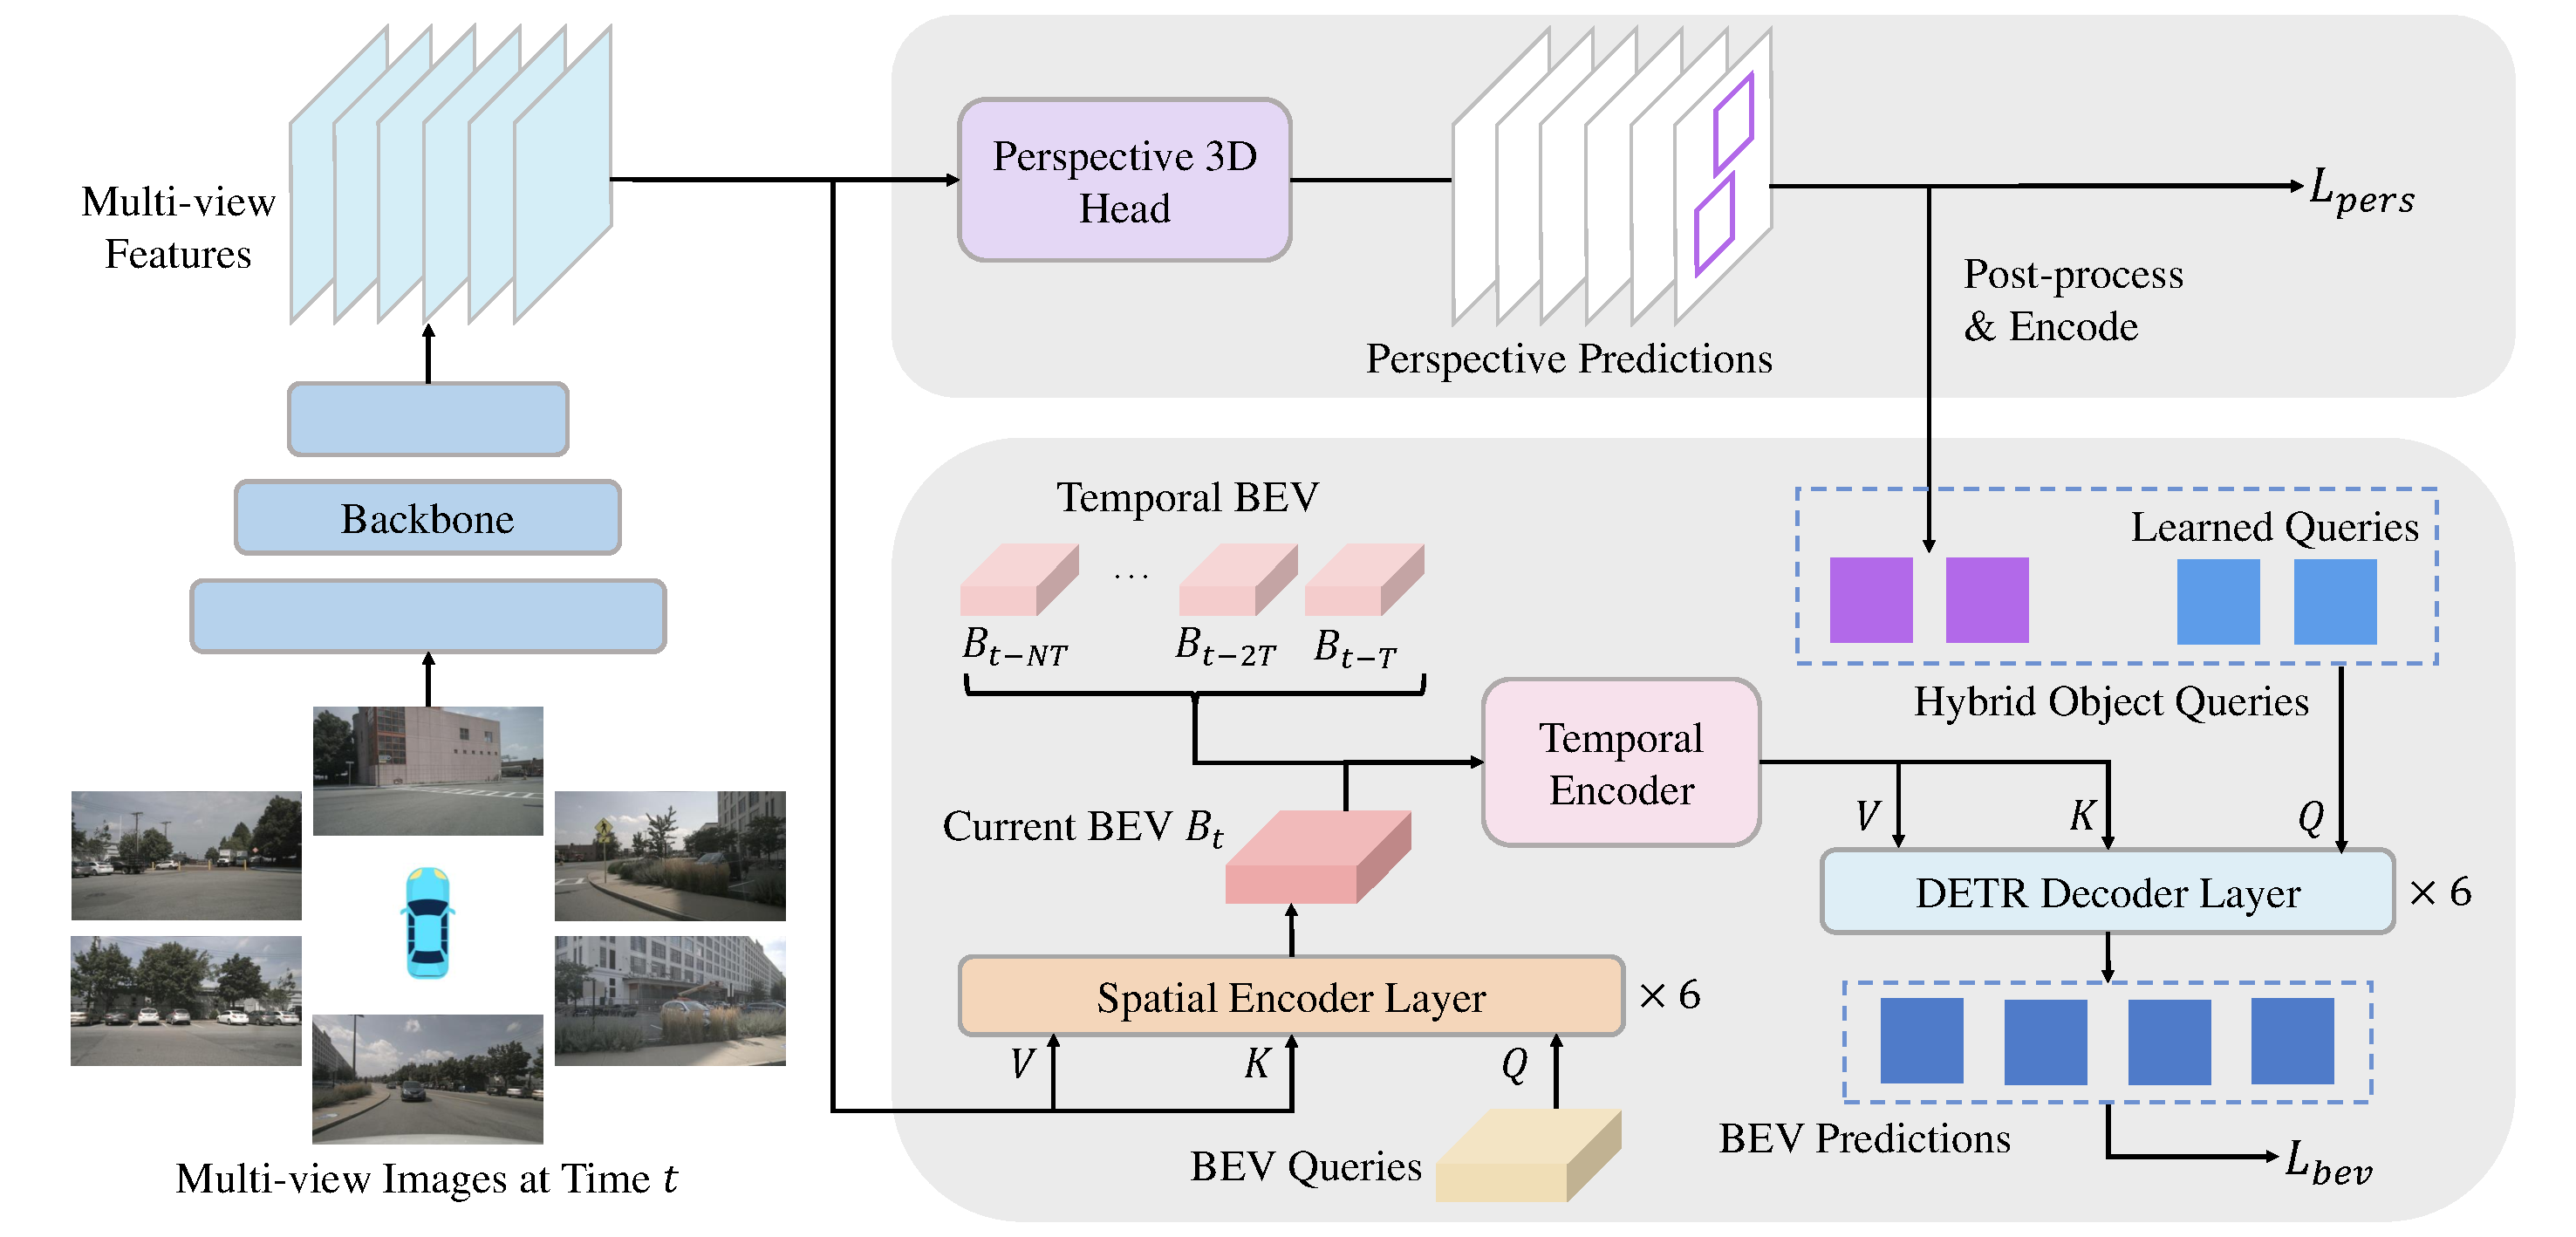
\includegraphics[width=0.9\textwidth]{figures/architecture2.pdf}
    \caption{BEVFormer v2 的整体架构。图像骨干网络提取多视角图像特征。透视3D头生成透视图预测，随后编码为物体查询（Object Query）。BEV头采用编码器-解码器（Encoder-Decoder）结构。空间编码器（Spatial Encoder）通过聚合多视角图像特征生成BEV特征，时序编码器（Temporal Encoder）收集历史BEV特征。解码器以混合物体查询（Hybrid Object Query）为输入，基于BEV特征生成最终BEV预测。整个模型使用两个检测头的损失项 $L_{pers}$ 和 $L_{bev}$ 进行训练。}
    \label{fig:architecture}
\end{figure*}

\subsection{相机3D目标检测中的辅助损失}
辅助损失（Auxiliary Loss）在单目3D目标检测中无处不在，因为大多数方法~\cite{MonoDIS,monoflex,fcos3d,DD3D,MonoCon,bevdepth,mv-fcos3d} 都建立在 RetinaNet~\cite{RetinaNet} 和 FCOS~\cite{fcos} 等2D检测器之上。
但这些辅助损失很少赋予2D监督任何明确的含义。
MonoCon~\cite{MonoCon} 充分利用了2D辅助损失，使用了多达5种不同的2D监督。
对于BEV检测器，BEVDepth~\cite{bevdepth} 利用 LiDAR 点云监督其中间深度网络。
MV-FCOS3D++~\cite{mv-fcos3d} 引入了透视监督（Perspective Supervision）用于训练其图像骨干网络，但检测器本身仅由BEV损失监督。
SimMOD~\cite{SimMOD} 为其单目提议头（Monocular Proposal Head）使用了2D辅助损失。

与先前方法不同，本文采用了端到端（End-to-end）的透视监督方法，无需使用 LiDAR 点云等额外数据。

\subsection{两阶段3D目标检测器}
尽管两阶段（Two-stage）检测器在基于 LiDAR 的3D目标检测中很常见~\cite{MV3D,AVOD,centerpoint,lidar-rcnn,frustum-pointnet,transfusion,SimMOD}，但其在基于相机的3D检测中的应用却鲜为人知。
MonoDIS~\cite{MonoDIS} 使用 RoIAlign 从2D框中提取图像特征并随后回归3D框。
SimMOD~\cite{SimMOD} 使用单目3D头生成提议，并使用 DETR3D \cite{DETR3D} 头进行最终检测。
然而，在两个阶段中使用来自透视骨干网络的相同特征，无法为第二阶段头提供信息增益。
本文推测这是两阶段检测器在基于相机的3D检测中不太受欢迎的主要原因。
相反，本文的两阶段检测器同时利用透视图和BEV视图的特征，从而兼顾了图像空间和BEV空间中的信息。

%\input{texts/3a-problem}
\section{BEVFormer v2}
将现代2D图像骨干网络（Image Backbone）适配到BEV识别中，无需繁琐的深度预训练（Depth Pre-training），将为下游自动驾驶任务开启许多可能性。
本文提出 BEVFormer v2，一种两阶段（Two-stage）BEV检测器，同时结合BEV和透视监督（Perspective Supervision），在BEV检测中无障碍地采用图像骨干网络。

\subsection{整体架构}
如图 \ref{fig:architecture} 所示，BEVFormer v2 主要由五个组件构成：图像骨干网络、透视3D检测头（Perspective 3D Detection Head）、空间编码器（Spatial Encoder）、改进的时序编码器（Temporal Encoder）和BEV检测头（BEV Detection Head）。
与原始 BEVFormer~\cite{bevformer} 相比，除空间编码器外所有组件均进行了修改。
具体而言，BEVFormer v2 使用的所有图像骨干网络均未使用任何自动驾驶数据集或深度估计数据集进行预训练。
引入透视3D检测头以促进2D图像骨干网络的适配，并为BEV检测头生成物体提议（Object Proposal）。
采用新的时序BEV编码器以更好地整合长期时序信息。
BEV检测头现在接收混合物体查询（Hybrid Object Query）集作为输入。本文将第一阶段提议与可学习物体查询结合，形成新的混合物体查询用于第二阶段。

\subsection{透视监督}
本文首先分析鸟瞰视图模型的问题，以解释为何需要额外的监督。
典型的BEV模型维护附着在BEV平面上的网格状特征，其中每个网格从多视角图像对应2D像素的特征中聚合3D信息。
模型基于BEV特征预测目标物体的3D边界框，本文将这种施加在BEV特征上的监督称为BEV监督（BEV Supervision）。
以 BEVFormer \cite{bevformer} 为例，其使用编码器-解码器结构生成和利用BEV特征。
编码器为BEV平面上的每个网格单元分配一组3D参考点（Reference Point），并将它们投影到多视角图像上作为2D参考点。
然后，在2D参考点周围采样图像特征，利用空间交叉注意力（Spatial Cross-attention）将其聚合为BEV特征。
解码器是一个可变形 DETR（Deformable DETR）\cite{deformable-detr} 头，使用少量固定数量的物体查询（Object Query）在BEV坐标系中预测3D边界框。
图 \ref{fig:supervision} 展示了由3D到2D视图变换和 DETR \cite{DETR} 头引入的BEV监督的两个潜在问题：
\begin{itemize}
    \item 监督对于图像特征是隐式的（Implicit）。损失直接作用于BEV特征，经过3D到2D的投影和图像特征的注意力采样后变为间接。
    \item 监督对于图像特征是稀疏的（Sparse）。只有少量被物体查询关注的BEV网格对损失有贡献，因此仅有这些网格的2D参考点周围的稀疏像素获得监督信号。
\end{itemize}
因此，训练中出现不一致性：BEV检测头依赖于图像特征中包含的3D信息，但骨干网络如何编码这些信息却缺少足够的指导。

\label{sec:perspective_supervision}
\begin{figure}[t]
    \centering
    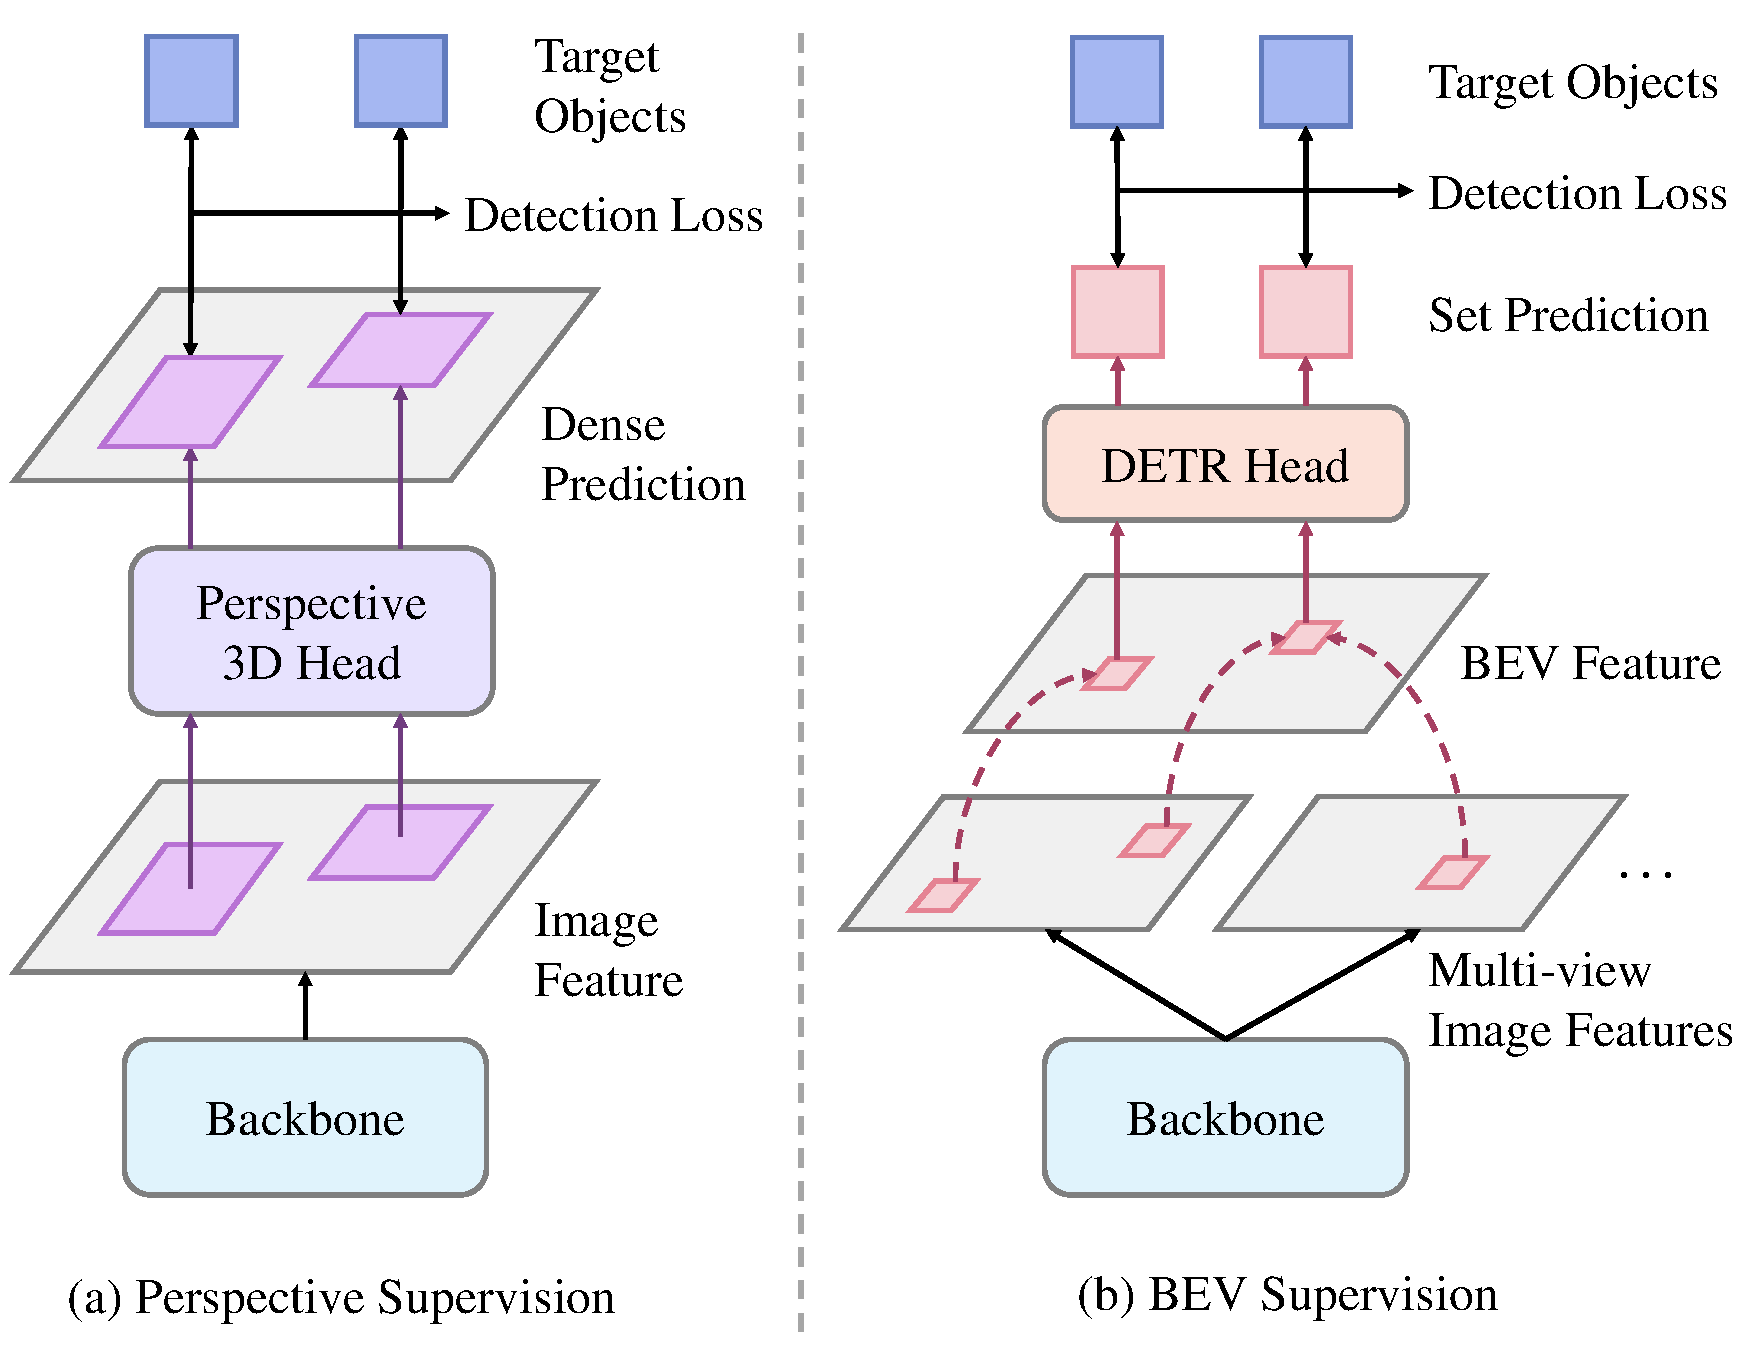
\includegraphics[width=1.0\linewidth]{figures/supervision.pdf}
    \caption{透视监督（a）与 BEV 监督（b）的对比。透视检测器的监督信号对图像特征是密集且直接的，而BEV检测器的监督信号则是稀疏且间接的。}
    \label{fig:supervision}
\end{figure}

先前的BEV方法并未严重受到此不一致性的影响，甚至可能未意识到该问题。
这是因为其骨干网络要么规模较小，要么已在带有单目检测头的3D检测任务上进行了预训练。
与BEV头相反，透视3D头在图像特征上进行逐像素预测，为适配2D图像骨干网络提供了更丰富的监督信号。
本文将施加在图像特征上的监督定义为透视监督。
如图 \ref{fig:supervision} 所示，与BEV监督不同，透视检测损失直接且密集地作用于图像特征。
本文认为透视监督显式地指导骨干网络感知3D场景并提取有用信息（例如物体的深度和朝向），克服了BEV监督的缺陷，因此在使用现代图像骨干网络训练BEV模型时至关重要。

\subsection{透视损失}
根据前述分析，透视监督是优化BEV模型的关键。
在 BEVFormer v2 中，本文通过辅助透视损失（Auxiliary Perspective Loss）引入透视监督。
具体而言，在骨干网络上构建一个透视3D检测头，用于在透视图上检测目标物体。
本文采用类似 FCOS3D~\cite{fcos3d} 的检测头，预测3D边界框的中心位置、尺寸、朝向和投影中心度（Projected Center-ness）。
该检测头的检测损失（称为透视损失 $\mathcal{L}_{pers}$）作为BEV损失 $\mathcal{L}_{bev}$ 的补充，促进骨干网络的优化。
整个模型的总目标函数为：
\begin{equation}
\mathcal{L}_{total} = \lambda_{bev}\mathcal{L}_{bev}+\lambda_{pers}\mathcal{L}_{pers}.
\end{equation}

\subsection{改进的时序编码器}
BEVFormer 使用循环时序自注意力（Recurrent Temporal Self-attention）来整合历史BEV特征。
但该时序编码器在利用长期时序信息方面存在不足，简单地将循环步数从4增加到16并不能带来额外的性能提升。

本文为 BEVFormer v2 重新设计了时序编码器，采用简单的扭曲拼接（Warp and Concatenate）策略。
给定不同帧 $k$ 的BEV特征 $B_k$，首先根据帧 $t$ 和帧 $k$ 之间的参考帧变换矩阵 $T_k^{t} = [\bf{R} | \bf{t}] \in \text{SE3}$，将 $B_k$ 双线性扭曲到当前帧得到 $B_k^t$。
然后沿通道维度拼接历史BEV特征与当前BEV特征，并使用残差块（Residual Block）进行降维。
为保持与原始设计相似的计算复杂度，本文使用相同数量的历史BEV特征但增加了采样间隔。
除了利用长期时序信息外，新的时序编码器还开启了在离线3D检测设置中利用未来BEV特征的可能性。

\subsection{两阶段BEV检测器}
尽管两个检测头的联合训练已经提供了足够的监督，但本文从不同视图各自获得两组检测结果。
本文并未采用直接使用BEV头的预测并丢弃透视图头的预测，或通过NMS启发式地合并两组预测的做法，而是设计了一种将两个头整合为两阶段预测流程的新颖结构，即两阶段BEV检测器。
BEV头中的物体解码器（Object Decoder）是一个 DETR \cite{DETR} 解码器，使用一组可学习的嵌入（Learned Embedding）作为物体查询，通过训练学习目标物体可能的位置。
然而，随机初始化的嵌入需要很长时间来学习合适的位置。
此外，学习到的物体查询在推理时对所有图像固定不变，由于物体的空间分布可能变化，这可能不够精准。
为解决这些问题，透视图头的预测经过后处理筛选后融合到解码器的物体查询中，形成两阶段流程。
这些混合物体查询提供了高分（高概率）的候选位置，使BEV头在第二阶段更容易捕捉目标物体。混合物体查询解码器的细节将在后文描述。
需要注意的是，第一阶段提议不一定来自透视检测器——例如可以来自另一个BEV检测器——但实验表明，只有来自透视图的预测对第二阶段BEV头有帮助。

\subsection{混合物体查询解码器}
为了将第一阶段提议融合到第二阶段的物体查询中，BEVFormer v2 中BEV头的解码器在 BEVFormer \cite{bevformer} 使用的可变形 DETR（Deformable DETR）\cite{deformable-detr} 解码器基础上进行了修改。
解码器由堆叠的交替自注意力（Self-attention）和交叉注意力（Cross-attention）层组成。
交叉注意力层是一个可变形注意力模块 \cite{deformable-detr}，接收以下三个元素作为输入：
(1) 内容查询（Content Query）——用于生成采样偏移和注意力权重的查询特征。
(2) 参考点（Reference Point）——值特征上的2D点，作为每个查询的采样参考。
(3) 值特征（Value Feature）——被关注的BEV特征。
在原始 BEVFormer \cite{bevformer} 中，内容查询是一组可学习的嵌入，参考点通过线性层从一组可学习的位置嵌入预测得到。
在 BEVFormer v2 中，本文从透视头获取提议，并通过后处理筛选部分提议。
%as described in ~\cref{sec/appendix/post-process}.
如图 \ref{fig:decoder} 所示，被选提议在BEV平面上投影的框中心用作逐图像参考点，并与从位置嵌入生成的逐数据集参考点相结合。
逐图像参考点直接指示物体在BEV平面上可能存在的位置，使解码器更容易检测目标物体。
然而，由于遮挡或出现在相邻视图边界，少量物体可能未被透视头检测到。
为避免遗漏这些物体，本文保留原始逐数据集参考点，通过学习空间先验来捕获它们。

\begin{figure}[t]
    \centering
    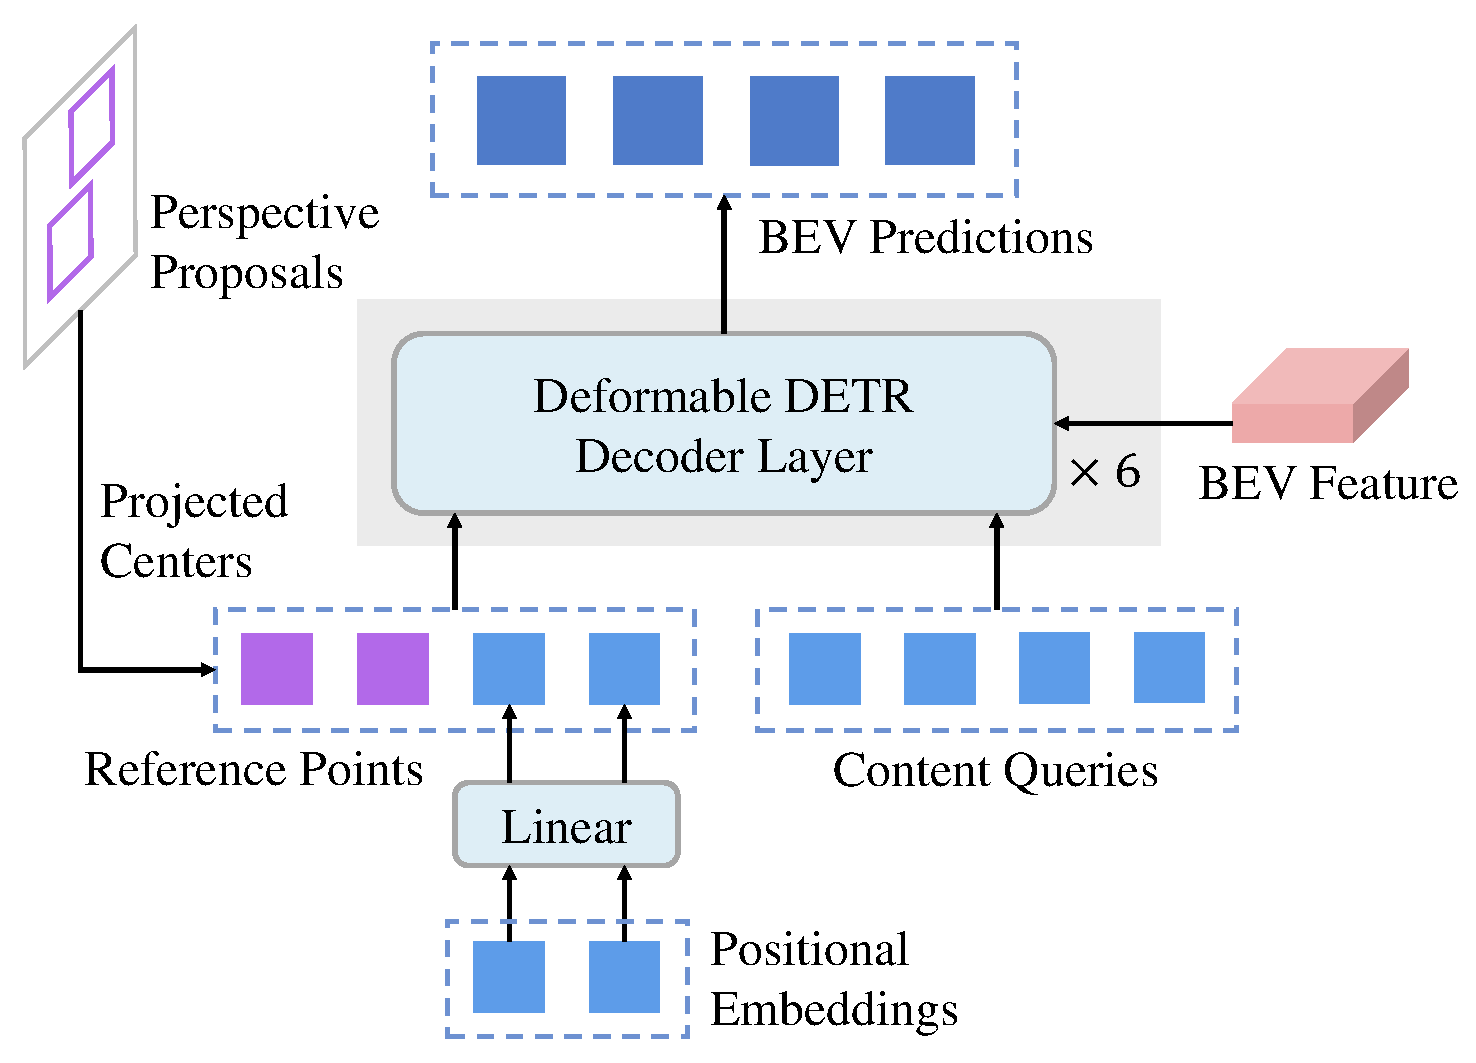
\includegraphics[width=1.0\linewidth]{figures/decoder.pdf}
    \caption{BEVFormer v2 中 BEV 头的解码器。第一阶段提议的投影中心用作逐图像参考点（紫色），与逐数据集学习的内容查询和位置嵌入（蓝色）结合为混合物体查询。}
    \label{fig:decoder}
    \vspace{-0.3cm}
\end{figure}

\section{实验}
\subsection{数据集与评估指标}
nuScenes 3D检测基准测试（Benchmark）\cite{nuscenes} 包含1000个多模态视频，每个视频时长约20秒，关键帧以2Hz频率标注。
每个样本包含来自6个相机的图像，覆盖360度全景视野。
视频分为700个训练、150个验证和150个测试。检测任务包含10个物体类别的140万个标注3D边界框。
nuScenes 使用地面平面上基于中心距离的四个不同阈值计算平均精度（Mean Average Precision, mAP），并包含五个真阳性指标：ATE（平移误差）、ASE（尺度误差）、AOE（朝向误差）、AVE（速度误差）和AAE（属性误差）。
此外，通过结合检测精度（mAP）与五个真阳性指标定义了 nuScenes 检测分数（NDS）。

\setlength{\tabcolsep}{3pt}
\setlength{\doublerulesep}{2\arrayrulewidth}
\renewcommand{\arraystretch}{1.1}
\begin{table*}[t]
    \caption{BEVFormer v2 与其他当前最优（SOTA）方法在 nuScenes 测试集上的3D检测结果。$^\dagger$ 表示 V2-99 \cite{Vovnet} 在深度估计（Depth Estimation）任务上使用额外数据 \cite{DD3D} 进行了预训练。$^\ddagger$ 表示使用 CBGS 的方法，该方法将1个epoch延长为4.5个epoch。本文仅训练 BEVFormer v2 24个epoch以与先前方法公平比较。}
    \label{table:sota_nuscenes}
    \centering

    \begin{tabular}{l|c|c|c|cc|ccccc}
        \toprule
        Method & Backbone & Epoch & Image Size & NDS & mAP & mATE & mASE & mAOE & mAVE & mAAE \\ 
        \midrule
        BEVFormer~\cite{bevformer} & V2-99$^\dagger$ & 24 & 900 $\times$ 1600 & 0.569 & 0.481 & 0.582 & 0.256 & 0.375 & 0.378 & 0.126 \\
        PolarFormer~\cite{polarformer} & V2-99$^\dagger$ & 24 & 900 $\times$ 1600 & 0.572 & 0.493 & 0.556 & 0.256 & 0.364 & 0.440 & 0.127 \\
        PETRv2~\cite{petrv2} & GLOM & 24 & 640 $\times$ 1600 & 0.582 & 0.490 & 0.561 & 0.243 & 0.361 & 0.343 & 0.120 \\
        BEVDepth~\cite{bevdepth} & V2-99$^\dagger$ & 90$^\ddagger$ & 640 $\times$ 1600 & 0.600 & 0.503 & 0.445 & 0.245 & 0.378 & 0.320 & 0.126 \\
        BEVStereo~\cite{bevstereo} & V2-99$^\dagger$ & 90$^\ddagger$ & 640 $\times$ 1600 & 0.610 & 0.525 & 0.431 & 0.246 & 0.358 & 0.357 & 0.138 \\
        \midrule
        \textbf{BEVFormer v2} & InternImage-B & 24 & 640 $\times$ 1600 & 0.620 & 0.540 & 0.488 & 0.251 & 0.335 & 0.302 & 0.122 \\
        \textbf{BEVFormer v2} & InternImage-XL & 24 & 640 $\times$ 1600 & 0.634 & 0.556 & 0.456 & 0.248 & 0.317 & 0.293 & 0.123 \\
        \bottomrule
    \end{tabular}

\end{table*}
\setlength{\tabcolsep}{3pt}
\setlength{\doublerulesep}{2\arrayrulewidth}
\renewcommand{\arraystretch}{1.1}
\begin{table*}[t]
    \caption{不同视图监督（View Supervision）组合的3D检测器在 nuScenes 验证集上的检测结果。所有模型均未使用时序（Temporal）信息训练。}
    \label{table:view_supervision}
    \centering

    \begin{tabular}{c|c|c|cc|cccccc}
        \toprule
        View Supervision & Backbone & Epoch & NDS & mAP & mATE & mASE & mAOE & mAVE & mAAE   \\ 
        \midrule 
        Perspective Only & ResNet-101 & 48 & 0.412 & 0.323 & 0.737 & 0.268 & 0.377 & 0.943 & 0.167 \\ 
        BEV Only & ResNet-101 & 48 & 0.426 & 0.355 & 0.751 & 0.275 & 0.429 & 0.847 & 0.215 \\ 
        Perspective \& BEV & ResNet-101 & 48 & 0.451 & 0.374 & 0.730 & 0.270 & 0.379 & 0.773 & 0.205 \\ 
        BEV \& BEV & ResNet-101 & 48 & 0.428 & 0.350 & 0.750 & 0.279 & 0.388 & 0.842 & 0.210 \\ 
        \midrule
        \bottomrule
    \end{tabular}
    
\end{table*}

\subsection{实验设置}
本文使用多种骨干网络进行实验：ResNet~\cite{ResNet}、DLA~\cite{DLA}、VoVNet~\cite{Vovnet} 和 InternImage \cite{InternImage}。
所有骨干网络均使用在 COCO 数据集 \cite{COCO} 的2D检测任务上预训练的检查点初始化。
除本文修改外，遵循 BEVFormer~\cite{bevformer} 的默认设置构建BEV检测头。
在表 \ref{table:sota_nuscenes} 和表 \ref{table:trick} 中，BEV头采用新的时序编码器利用时序信息。其他实验中，采用仅使用当前帧的单帧版本，类似 BEVFormer-S~\cite{bevformer}。
对于透视3D检测头，采用 DD3D~\cite{DD3D} 的实现，带有相机感知深度参数化（Camera-aware Depth Parameterization）。
透视损失和BEV损失的权重设为 $\lambda_{bev}=\lambda_{pers}=1$。
使用 AdamW~\cite{AdamW} 优化器，基础学习率设为 4e-4。

\subsection{基准测试结果}
本文将提出的 BEVFormer v2 与现有当前最优（SOTA）的BEV检测器进行比较，包括 BEVFormer~\cite{bevformer}、PolarFormer~\cite{polarformer}、PETRv2~\cite{petrv2}、BEVDepth~\cite{bevdepth} 和 BEVStereo~\cite{bevstereo}。
表 \ref{table:sota_nuscenes} 报告了 nuScenes 测试集上的3D目标检测结果。
BEVFormer、PolarFormer、BEVDepth 和 BEVStereo 使用的 V2-99 \cite{Vovnet} 骨干网络已在额外数据的深度估计任务上预训练，然后通过 DD3D \cite{DD3D} 在 nuScenes 数据集 \cite{nuscenes} 上微调。
相反，本文采用的 InternImage \cite{InternImage} 骨干网络使用来自 COCO~\cite{COCO} 检测任务的检查点初始化，没有任何3D预训练。
InternImage-B 的参数量与 V2-99 相似，但更能体现现代图像骨干网络设计的进步。
可以观察到，使用 InternImage-B 骨干网络的 BEVFormer v2 优于所有现有方法，表明在透视监督下，不再需要单目3D任务预训练的骨干网络。
使用 InternImage-XL 的 BEVFormer v2 以 63.4\% NDS 和 55.6\% mAP 超越了 nuScenes 相机3D目标检测排行榜上的所有方法，比第二名 BEVStereo 高出 2.4\% NDS 和 3.1\% mAP。
这一显著提升揭示了释放现代图像骨干网络在BEV识别中的巨大潜力所带来的收益。

\setlength{\tabcolsep}{3pt}
\setlength{\doublerulesep}{2\arrayrulewidth}
\renewcommand{\arraystretch}{1.1}
\begin{table*}[ht]
    \caption{透视监督（Perspective Supervision）在不同2D图像骨干网络（Image Backbone）上的结果，在 nuScenes 验证集上评测。"BEV Only" 和 "Perspective \& BEV" 与表 \ref{table:view_supervision} 相同。所有骨干网络均使用 COCO~\cite{COCO} 预训练权重初始化，所有模型均未使用时序（Temporal）信息训练。}
    \label{table:large_backbone}
    \centering

    \begin{tabular}{c|c|c|cc|cccccc}
        \toprule
        Backbone & Epoch & View Supervision & NDS & mAP & mATE & mASE & mAOE & mAVE & mAAE   \\ 
        \midrule
        ResNet-50 & 48 & BEV Only & 0.400 & 0.327 & 0.795 & 0.277 & 0.479 &0.871 & 0.210 \\ 
        ResNet-50 & 48 & Perspective \& BEV & 0.428 & 0.349 & 0.750 & 0.276 & 0.424 & 0.817 & 0.193 \\
        \midrule
        DLA-34 & 48 & BEV Only & 0.403 & 0.338 & 0.772 & 0.279 & 0.483 & 0.919 & 0.206 \\ 
        DLA-34 & 48 & Perspective \& BEV & 0.435 & 0.358 & 0.742 & 0.274 & 0.431 & 0.801 & 0.186 \\  
  
        \midrule
        ResNet-101 & 48 & BEV Only & 0.426 & 0.355 & 0.751 & 0.275 & 0.429 & 0.847 & 0.215  \\ 
        ResNet-101 & 48 & Perspective \& BEV & 0.451 & 0.374 & 0.730 & 0.270 & 0.379 & 0.773 & 0.205  \\   
        \midrule
        VoVNet-99 & 48 & BEV Only & 0.441 & 0.367  & 0.734 & 0.271 & 0.402 & 0.815  & 0.205 \\ 
        VoVNet-99 & 48 & Perspective \& BEV & 0.467 & 0.396  & 0.709  & 0.274 & 0.368 & 0.768 & 0.196 \\ 
        \midrule
        InternImage-B & 48 & BEV Only & 0.455 & 0.398  & 0.712 & 0.283 & 0.411 & 0.826  & 0.204 \\ 
        InternImage-B & 48 & Perspective \& BEV & 0.485 & 0.417  & 0.696  & 0.275 & 0.354 & 0.734 & 0.182 \\ 
        \bottomrule
    \end{tabular}
    
\end{table*}
\setlength{\tabcolsep}{3pt}
\setlength{\doublerulesep}{2\arrayrulewidth}
\renewcommand{\arraystretch}{1.1}
\begin{table*}[t]
    \caption{仅使用 BEV 监督（BEV Supervision）与同时使用透视和 BEV 监督（Perspective \& BEV Supervision）的模型在不同训练轮数下的对比。模型在 nuScenes 验证集上评测。所有模型均未使用时序（Temporal）信息训练。}
    \label{table:long_schedule}
    \centering

    \begin{tabular}{c|c|c|cc|cccccc}
        \toprule
        View Supervision & Backbone & Epoch  & NDS & mAP & mATE & mASE & mAOE & mAVE & mAAE   \\ 
        \midrule 
        \multirow{3}{*}{BEV Only} & \multirow{3}{*}{ResNet-50} & 24 & 0.379 & 0.322 & 0.803 & 0.280 & 0.549 & 0.954 & 0.240 \\ 
         &  & 48 & 0.400 & 0.327 & 0.795 & 0.277 & 0.479 & 0.871 & 0.210 \\ 
         &  & 72 & 0.410 & 0.335 & 0.771 & 0.280 & 0.458 & 0.848 & 0.216 \\ 
        \midrule
        \multirow{3}{*}{Perspective \& BEV} & \multirow{3}{*}{ResNet-50} & 24 &  0.414 & 0.351 & 0.732 & 0.271 & 0.505 & 0.899 & 0.204 \\ 
         &  & 48 & 0.428 & 0.349 & 0.750 & 0.276 & 0.424 & 0.817 & 0.193 \\ 
         &  & 72 & 0.428 & 0.351 & 0.741 & 0.279 & 0.419 & 0.835 & 0.196 \\ 
        \midrule
        \bottomrule
    \end{tabular}
\end{table*}
%\vspace{+5pt}

\subsection{消融实验与分析}
\subsubsection{透视监督的有效性}
为验证透视监督的有效性，本文在表 \ref{table:view_supervision} 中比较了不同视图监督组合的3D检测器，包括：
(1) 透视与BEV（Perspective \& BEV）——本文提出的 BEVFormer v2，整合了透视头和BEV头的两阶段检测器。
(2) 仅透视（Perspective Only）——本文模型中的单阶段透视检测器。
(3) 仅BEV（BEV Only）——本文模型中不使用混合物体查询的单阶段BEV检测器。
(4) BEV与BEV（BEV \& BEV）——具有两个BEV头的两阶段检测器，即将本文模型中的透视头替换为另一个利用BEV特征生成混合物体查询提议的BEV头。

与仅透视检测器相比，仅BEV检测器通过利用多视角图像实现了更好的NDS和mAP，但其mATE和mAOE更高，表明了BEV监督的潜在问题。
本文的透视与BEV检测器实现了最佳性能，分别超过仅BEV检测器2.5\% NDS和1.9\% mAP。
具体而言，透视与BEV检测器的mATE、mAOE和mAVE显著低于仅BEV检测器。
这一显著提升主要来自以下两个方面：
(1) 在常规视觉任务上预训练的骨干网络无法捕获3D场景中物体的某些属性，包括深度、朝向和速度，而受透视监督指导的骨干网络能够提取这些属性的信息。
(2) 与固定物体查询集相比，本文的混合物体查询包含第一阶段预测作为参考点，帮助BEV头定位目标物体。
为进一步确保提升并非来自两阶段流程本身，本文引入BEV与BEV检测器进行比较。
结果表明，BEV与BEV检测器与仅BEV检测器表现相当，远不及透视与BEV检测器。
因此，仅在透视图上构建第一阶段头并施加辅助监督对BEV模型是有帮助的。

%\vspace{-0.3cm}
\subsubsection{透视监督的泛化性}
本文提出的透视监督预期适用于不同架构和大小的骨干网络。
本文在一系列常用于3D目标检测任务的骨干网络上构建 BEVFormer v2：ResNet \cite{ResNet}、DLA \cite{DLA}、VoVNet \cite{Vovnet} 和 InternImage \cite{InternImage}。结果报告在表 \ref{table:large_backbone} 中。
与纯BEV检测器相比，BEVFormer v2（BEV与透视）在所有骨干网络上的NDS提升约3\%，mAP提升约2\%，表明其适用于不同架构和模型大小。
本文认为额外的透视监督可以成为训练BEV模型的通用方案，特别是在没有3D预训练的情况下适配大规模图像骨干网络时。

\setlength{\tabcolsep}{3pt}
\setlength{\doublerulesep}{2\arrayrulewidth}
\renewcommand{\arraystretch}{1.1}
\begin{table*}[ht]
    \caption{BEVFormer v2 中透视图头（Perspective Head）与 BEV 头（BEV Head）不同选择的对比。模型在 nuScenes 验证集上评测。所有模型均未使用时序（Temporal）信息训练。}
    \label{table:detector_choice_for_two_view}
    \centering
    \vspace{-5pt}
    \begin{tabular}{cc|c|c|cc|ccccc}
        \toprule
        Perspective View & BEV View & Backbone & Epoch & NDS & mAP & mATE & mASE & mAOE & mAVE & mAAE   \\ 
        \midrule 
        DD3D & Deformable DETR & ResNet-50 & 48 & 0.428 & 0.349 & 0.750 & 0.276 & 0.424 & 0.817 & 0.193 \\ 
        DD3D & Group DETR & ResNet-50 & 48 & 0.445 & 0.353 & 0.725 & 0.276 & 0.366 & 0.767 & 0.180 \\ 
         DETR3D & Deformable DETR & ResNet-50 & 48 & 0.409 & 0.335 & 0.765 & 0.276 & 0.469 & 0.877 & 0.198 \\ 
        DETR3D & Group DETR & ResNet-50 & 48 & 0.423 & 0.351 & 0.743 & 0.279 & 0.466 & 0.844 & 0.201 \\ 
        \midrule
        \bottomrule
    \end{tabular}
    
\end{table*}
\let\ck\checkmark

\setlength{\tabcolsep}{3pt}
\setlength{\doublerulesep}{2\arrayrulewidth}
\renewcommand{\arraystretch}{1.0}
\begin{table*}[t]
    \caption{BEVFormer v2 各组件（Bells and Whistles）的消融实验（Ablation Study），在 nuScenes 验证集上评测。所有模型均使用 ResNet-50 骨干网络（Backbone）及时序（Temporal）信息训练。`Pers'、`IDA'、`Long' 和 `Bi' 分别表示透视监督（Perspective Supervision）、图像级数据增强（Image-level Data Augmentation）、长时序间隔（Long Temporal Interval）和双向时序编码器（Bi-directional Temporal Encoder）。}
    \label{table:trick}
    \centering
    \vspace{-5pt}
    \begin{tabular}{l|c|cccc|cc|cc|cccccc}
        \toprule
        Method & Epoch & Pers & IDA & Long & Bi & NDS & mAP & mATE & mASE & mAOE & mAVE & mAAE   \\ 
        \midrule
        Baseline & 24 & \ck & & & & 0.478 & 0.368 & 0.709 & 0.282 & 0.452 & 0.427 & 0.191 \\ 
        Image-level Data Agumentation & 24 & \ck & \ck & & & 0.489 & 0.386 & 0.690 & 0.273 & 0.482 & 0.395 & 0.199 \\
        % BDA  & & & & & & & \\
        Longer Temporal Interval & 24 & \ck & \ck & \ck & & 0.498 & 0.388 & 0.679 & 0.276 & 0.417 & 0.403 & 0.189 \\
        % Randomized Temporal   & \ck & \ck & \ck & \ck & & & \\ 
        Bi-directional Temporal Encoder & 24 & \ck & \ck & \ck & \ck & 0.529 & 0.423 & 0.618 & 0.273 & 0.413 & 0.333 & 0.181 \\
        All but Perspective & 24 & & \ck & \ck & \ck & 0.507 & 0.397 & 0.636 & 0.281 & 0.455 & 0.356 & 0.190 \\
        \bottomrule
    \end{tabular}
    
\end{table*}

\subsubsection{训练轮数的选择}
本文对仅BEV模型和 BEVFormer v2（BEV与透视）进行了不同轮数的训练，观察两个模型达到收敛所需的时间。
表 \ref{table:long_schedule} 显示，本文的BEV与透视模型比仅BEV模型收敛更快，证实了辅助透视损失促进了优化。
仅BEV模型在更长时间的训练下仅获得边际提升。
但在72个epoch时两个模型之间的差距仍然存在，且即使更长时间的训练也可能无法消除，这表明仅靠BEV监督无法很好地适配图像骨干网络。
根据表 \ref{table:long_schedule}，本文模型训练48个epoch就已足够，其他实验除非另有说明均保持此设置。

\subsubsection{检测头的选择}
BEVFormer v2 可使用多种类型的透视和BEV检测头。
本文探索了几种代表性方法以选择最佳组合：对于透视头，候选方案为 DD3D \cite{DD3D} 和 DETR3D \cite{DETR3D}；对于BEV头，候选方案为可变形 DETR \cite{deformable-detr} 和 Group DETR \cite{groupdetr}。
DD3D 是一个单阶段无锚框（Anchor-free）透视头，在图像特征上进行密集的逐像素预测。
相反，DETR3D 使用3D到2D查询来采样图像特征并提出稀疏的预测集。
然而，根据本文的定义，它属于透视监督，因为它利用图像特征进行最终预测而不生成BEV特征，即损失直接作用于图像特征。
如表 \ref{table:detector_choice_for_two_view} 所示，DD3D 作为透视头优于 DETR3D，支持了本文在章节 \ref{sec:perspective_supervision} 中的分析。
DD3D 提供的密集直接监督对BEV模型有帮助，而 DETR3D 的稀疏监督无法克服BEV头的缺陷。
Group DETR 头是可变形 DETR 头的扩展，使用分组物体查询和组内自注意力。
Group DETR 在BEV头上取得了更好的性能，但计算量更大。
因此，本文在表 \ref{table:sota_nuscenes} 中采用了 DD3D 头和 Group DETR 头，在其他消融实验中保持与 BEVFormer \cite{bevformer} 相同的可变形 DETR 头。

%\vspace{-10pt}
\subsubsection{各组件的消融实验}
\label{sec:bells_and_whistles}
在表 \ref{table:trick} 中，本文对 BEVFormer v2 中采用的各种组件进行了消融实验，以确认其对最终结果的贡献，包括：
(1) 图像级数据增强（Image-level Data Augmentation, IDA）——图像随机水平翻转。
(2) 更长时序间隔——BEVFormer \cite{bevformer} 使用0.5秒间隔的连续帧，而本文的 BEVFormer v2 以2秒间隔采样历史BEV特征。
(3) 双向时序编码器（Bi-directional Temporal Encoder）——对于离线3D检测，本文 BEVFormer v2 中的时序编码器可以利用未来的BEV特征。
通过更长的时序间隔，模型可以从更多不同时间戳的自车位置收集信息，有助于估计物体朝向并显著降低mAOE。
在离线3D检测设置中，双向时序编码器能够提供来自未来帧的额外信息，大幅提升模型性能。
本文还在应用所有组件的情况下对透视监督进行了消融实验。
如表 \ref{table:trick} 所示，透视监督将NDS提升了2.2\%，mAP提升了2.6\%，是主要改进来源。

\section{结论}
现有工作在设计和改进鸟瞰视图（BEV）识别模型的检测器方面付出了大量努力，但它们通常局限于特定的预训练骨干网络，未进一步探索。
本文旨在释放现代图像骨干网络（Image Backbone）在BEV模型上的全部潜力。
本文将通用2D图像骨干网络适配的困难归因于BEV检测器的优化问题。
为解决此问题，本文通过从额外的透视3D检测头添加辅助损失（Auxiliary Loss），将透视监督（Perspective Supervision）引入BEV模型。
此外，本文将两个检测头整合为两阶段（Two-stage）检测器，即 BEVFormer v2。
功能完整的透视头提供第一阶段物体提议（Object Proposal），编码为BEV头的物体查询（Object Query）用于第二阶段预测。
大量实验验证了本文方法的有效性和泛化性。
透视监督引导2D图像骨干网络感知自动驾驶的3D场景，帮助BEV模型实现更快的收敛和更好的性能，并且适用于广泛的骨干网络。
此外，本文成功将大规模骨干网络适配到 BEVFormer v2，在 nuScenes 数据集上取得了新的SOTA结果。
本文的工作为未来研究者探索更好的BEV模型图像骨干网络设计铺平了道路。

\noindent\textbf{局限性.} 由于计算和时间限制，本文目前未在更大规模的图像骨干网络上测试方法。本文已在多种骨干网络上完成了初步验证，未来将扩展到更大的模型规模。


%%%%%%%%% REFERENCES
{\small
\bibliographystyle{ieee_fullname}
\bibliography{egbib}
}

%%%%%%%%% APPENDIX
\appendix
\clearpage
\section{实现细节}
本节提供所提方法和实验的更多实现细节。

\subsection{训练设置}
在表 \ref{table:training_setting_main} 中，提供了 BEVFormer v2 在 \cref{table:sota_nuscenes} 中用于 InternImage-B~\cite{InternImage} 和 InternImage-XL 骨干网络的超参数和训练方案。

\let\ck\checkmark

\setlength{\tabcolsep}{5pt}
\setlength{\doublerulesep}{2\arrayrulewidth}
\renewcommand{\arraystretch}{1.0}
\begin{table}[ht]
    \caption{BEVFormer v2 使用 InternImage 骨干网络（Backbone）的主要结果训练设置。}
    \label{table:training_setting_main}
    \centering
    \begin{tabular}{l|cc}
        %\toprule
        backbone & InternImage-B & InternImage-XL \\
        \hline
        training epochs & 24 & 24 \\
        batch size & 16 & 32 \\
        optimizer & AdamW & AdamW \\
        base learning rate & 4e-4 & 5e-4 \\
        weight decay & 0.01 & 0.01 \\
        lr schedule & step decay & step decay\\
        layer-wise lr decay & 0.96 & 0.94 \\
        warmup iters & 2000 & 2000  \\
        warmup schedule & linear & linear \\
        gradient clip & 35 & 35 \\
        \hline
        image size & 640 $\times$ 1600 & 640 $\times$ 1600 \\
        IDA & \ck & \ck \\
        temporal interval & 4 seconds & 4 seconds \\
        bi-directional & \ck & \ck \\
        \hline
    \end{tabular}
    
\end{table}

在表 \ref{table:large_backbone} 中，本文还在其他骨干网络上构建了 BEVFormer v2 检测器，包括 ResNet-50~\cite{ResNet}、DLA-34~\cite{DLA}、ResNet-101~\cite{ResNet} 和 VoVNet-99~\cite{Vovnet}。其训练设置列于表 \ref{table:training_setting_other}。

\let\ck\checkmark

\setlength{\tabcolsep}{5pt}
\setlength{\doublerulesep}{2\arrayrulewidth}
\renewcommand{\arraystretch}{1.0}
\begin{table}[ht]
    \caption{BEVFormer v2 使用其他骨干网络（Backbone）的训练设置。}
    \label{table:training_setting_other}
    \centering
    \begin{tabular}{l|cccc}
        %\toprule
        backbone & R50 & DLA34 & R101 & V2-99 \\
        \hline
        batch size & \multicolumn{4}{c}{16} \\
        optimizer & \multicolumn{4}{c}{AdamW} \\
        base lr & \multicolumn{4}{c}{4e-4} \\
        backbone lr & 2e-4 & 2e-4 & 4e-5 & 4e-5 \\
        weight decay & \multicolumn{4}{c}{0.01} \\
        \hline
    \end{tabular}
    
\end{table}

\subsection{网络架构}
在 BEVFormer v2 中，图像骨干网络产生步长为8、16和32的3层特征图。本文在骨干网络后采用FPN（特征金字塔网络）\cite{FPN} 生成步长为8、16、32、64和128的5层特征。透视头使用全部5层特征，而BEV头使用前4层（步长为8、16、32和64）。

\noindent\textbf{透视头.} 本文采用 DD3D~\cite{DD3D} 实现的单阶段无锚框（Anchor-free）单目3D检测器，包含三个独立头：分类头（Classification Head）、2D检测头（2D Detection Head）和3D检测头（3D Detection Head）。
分类头生成每个物体类别的 logit。
2D头通过特征位置到边界的4个偏移量生成与类别无关的边界框，并产生2D中心度（Center-ness）。
2D检测损失 $\mathcal{L}_{2D}$ 源自 FCOS~\cite{fcos}。
3D头预测3D边界框，包含以下系数：异体朝向（Allocentric Orientation）的旋转角、框中心深度、特征位置到投影框中心的偏移量，以及相对于类别典型尺寸的尺寸偏差。
此外，3D头生成预测3D框相对于2D置信度的置信度。
它采用 \cite{MonoDIS} 中的解耦 L1 损失（Disentangled L1 Loss）用于3D边界框回归，以及自监督损失（Self-supervised Loss）用于3D置信度，分别记为 $\mathcal{L}_{3D}$ 和 $\mathcal{L}_{conf}$。
BEVFormer v2 的透视损失是2D检测损失、3D回归损失和3D置信度损失之和：
\begin{equation}
    \mathcal{L}_{pers} = \mathcal{L}_{2D} + \mathcal{L}_{3D} + \mathcal{L}_{conf}
\end{equation}
透视检测头的更多细节请参见 \cite{DD3D}。

\begin{figure*}[t]
    \centering
    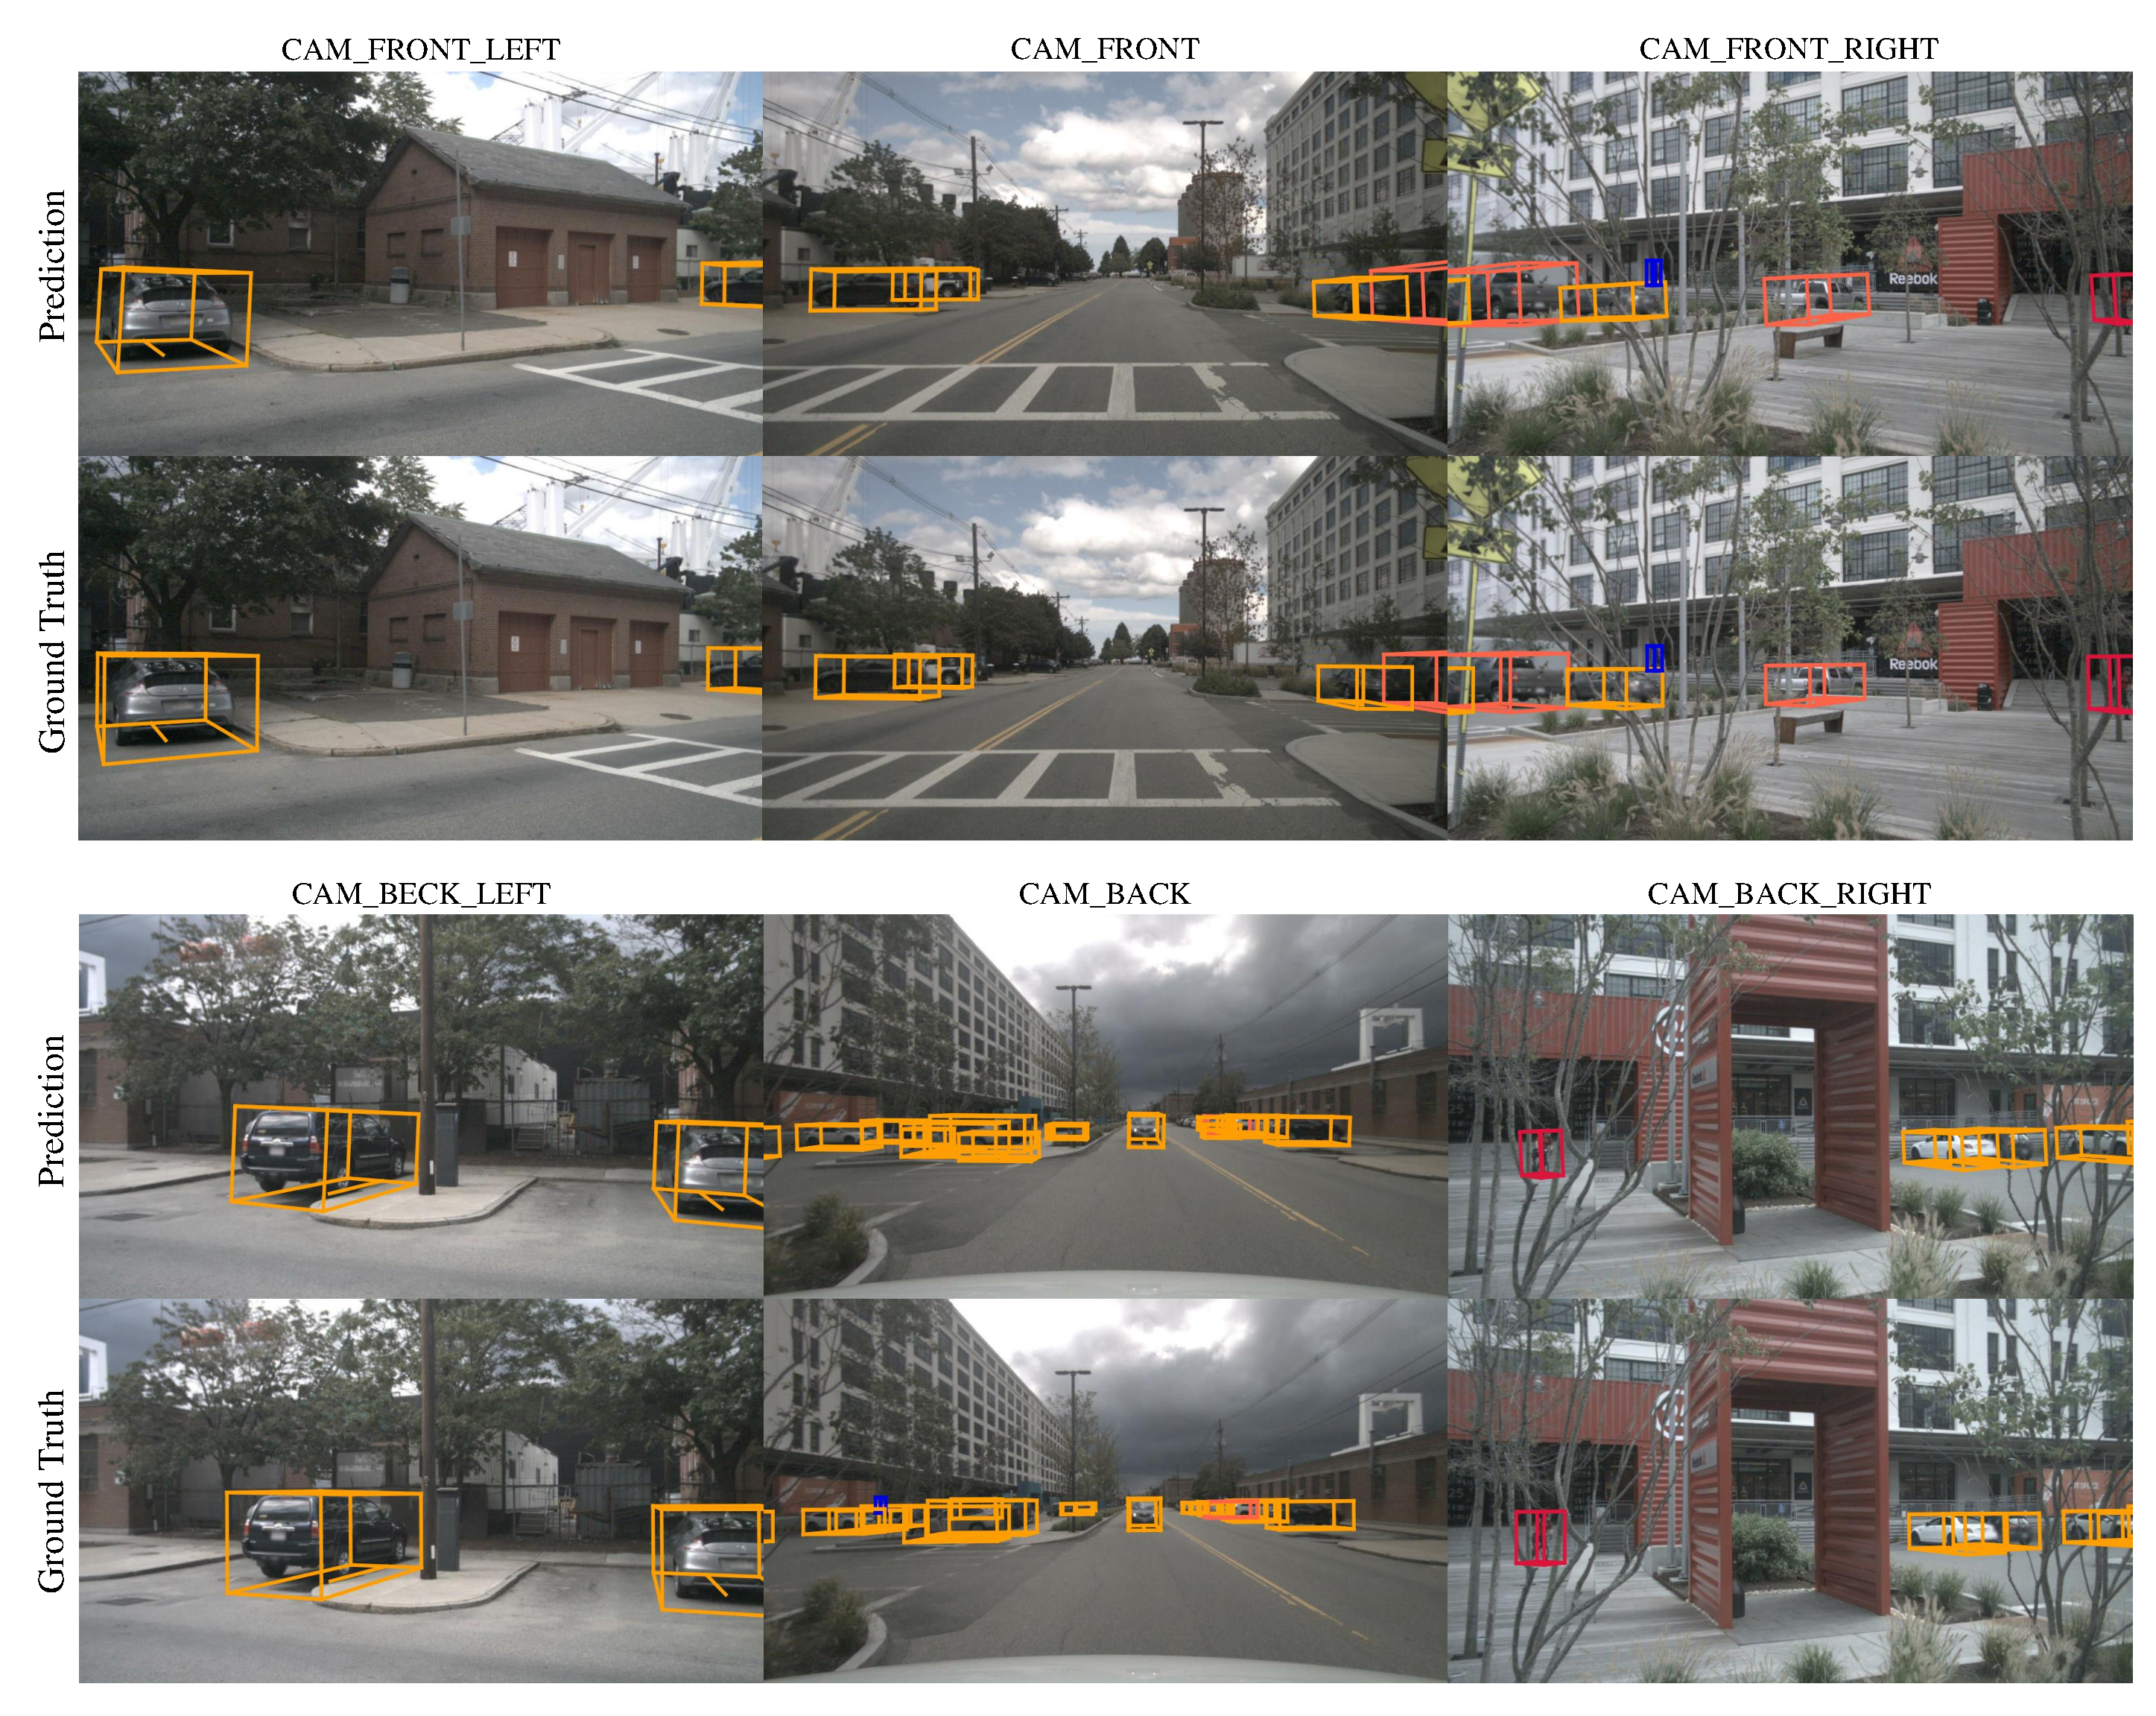
\includegraphics[width=0.8\textwidth]{figures/visualization2.pdf}
    \caption{BEVFormer v2 3D目标检测预测的可视化结果。}
    \label{fig:visualization}
\end{figure*}

\subsection{第一阶段提议的后处理}
\label{sec/appendix/post-process}
本节描述来自透视检测头的提议的后处理流程。
从透视头提供的所有相机视图的原始预测开始。
对于所有视图 $\mathcal{V}$ 中的第 $i$ 个视图，预测的3D边界框及其分数记为 $\{(\mathbf{B}_{i,j},s_{i,j})\}_j$。
通过以下后处理流程筛选出分数最高的候选。
首先，对每个视图 $i$ 的提议执行非极大值抑制（Non-maximum Suppression, NMS），以获取在透视图上无重叠的候选 $C_i$：
\begin{equation}
    C_i := \text{NMS}_{pers}\left(\{(\mathbf{B}_{i,j},s_{i,j})\}_j\right)
\end{equation}
NMS阈值设置为 2D IoU = 0.75。为确保所有相机视图中的物体都能被检测到，通过取每个视图 $i$ 在NMS后的 top-$k_1$ 来平衡不同视图的提议数量：
\begin{equation}
    C := \bigcup_{i\in\mathcal{V}} \text{top-}k_1\left(C_i\right)
\end{equation}
实验中设 $k_1=100$。
$C$ 中所有3D框通过相应的相机外参投影到鸟瞰视图坐标。
为避免出现在多个视图中的物体导致提议重叠，在BEV平面上以 BEV IoU = 0.3 应用另一个NMS：
\begin{equation}
    C := \text{NMS}_{bev}(C)
\end{equation}
最后，选择 top $k_2=100$ 个提议：
\begin{equation}
    C := \text{top-}k_2(C)
\end{equation}
对于最终提议集 $C$ 中的每个3D边界框 $\mathbf{B}$，其在BEV平面上的投影中心 $(c_x(\mathbf{B}),c_y(\mathbf{B}))$ 用作物体解码器中可变形 DETR 的参考点。


\section{可视化}
本文在 \cref{fig:visualization} 中展示了 BEVFormer v2 检测器的3D目标检测结果可视化。即使对于远处或被遮挡的困难样本，模型也能预测出准确的目标3D边界框。例如，模型成功检测到了前右相机远处的行人、后相机中与多辆车重叠的卡车，以及后右相机中被树遮挡的自行车。

% \section{进一步实证研究}
% \subsection{与深度预训练图像骨干网络的比较}
% To demonstrate that BEVFormer v2 does not require domain-specific pre-training to achieve SoTA results with large-scale image backbones, we compare BEVFormer v2 with the original BEVFormer~\cite{bevformer} using the DLA-34~\cite{DLA} and the VoVNet-99~\cite{Vovnet} backbones with different pre-training settsings in ~\cref{table:depth_pretrain}.
% \setlength{\tabcolsep}{3pt}
\setlength{\doublerulesep}{2\arrayrulewidth}
\renewcommand{\arraystretch}{1.0}
\begin{table*}[t]
    \caption{BEVFormer v2 在使用 COCO 预训练和深度预训练（Depth Pre-training）的 VoVNet-99 骨干网络时，在 nuScenes 测试集上的3D检测结果。省略 COCO 预训练的epoch数，因为 COCO 预训练骨干网络广泛可用且两种设置使用相同的 COCO 预训练。}
    \label{table:depth_pretrain}
    \centering

    \begin{tabular}{c|c|c|cc|cccccc}
        \toprule
        Backbone & Epoch & Pre-train & NDS & mAP & mATE & mASE & mAOE & mAVE & mAAE   \\ 
        \midrule
        DLA-34 & 72 & COCO & & & & & & & & \\ 
        DLA-34 & \small{15M Img + 120 + 24} & \small{COCO $\xrightarrow{}$ DDAD15M $\xrightarrow{}$ nuScenes} & & & & & & & \\ 
        \midrule
        VoVNet-99 & 72 & COCO & & & & & & & & \\ 
        VoVNet-99 & \small{15M Img + 120 + 24} & \small{COCO $\xrightarrow{}$ DDAD15M $\xrightarrow{}$ nuScenes} & & & & & & & \\ 
        \bottomrule
    \end{tabular}
\end{table*}

% \subsection{大规模图像骨干网络在长训练计划下的性能}
% \setlength{\tabcolsep}{3pt}
\setlength{\doublerulesep}{2\arrayrulewidth}
\renewcommand{\arraystretch}{1.0}
\begin{table*}[ht]
    \caption{InternImage-XL 在延长训练计划下，在 nuScenes 测试集上的3D检测结果。}
    \label{table:extend_training}
    \centering

    \begin{tabular}{c|c|cc|cccccc}
        \toprule
        Backbone & Epoch & NDS & mAP & mATE & mASE & mAOE & mAVE & mAAE   \\ 
        \midrule
        InternImage-XL & 24 & & & & & & & \\ 
        InternImage-XL & 48 & & & & & & & \\ 
        InternImage-XL & 72 & & & & & & & \\ 
        \bottomrule
    \end{tabular}
    
\end{table*}


\end{document}
